\subsection{Kinematic-wave columns (\texttt{KINEMATIC})}\label{sec:szvadosekw}
\cmd{:SoilZoneVadose KINEMATIC} $\epsilon$ $N$ replaces Richards' equation in the unsaturated columns by a gravity-only
kinematic wave, the approach of MODFLOW's UZF package and GSFLOW \cite{markstrom2008gsflow}. It still delays and spreads
recharge through a deep unsaturated zone with a travel time that depends on the flux, at a fraction of the cost, and it
cannot fail to converge. It has no parameter of its own: \emph{KINEMATIC is Richards without capillarity}, on the same
column (grid, materials, hotstart, water-table following, accounting) as Section~\ref{sec:szvadose}.

\paragraph{Equations.} With the capillary term dropped, Richards' equation becomes
\begin{equation}
\frac{\partial\theta}{\partial t}+\frac{\partial K(\theta)}{\partial z'}=0\qquad(z'\text{ downward}),
\end{equation}
with the column's own Campbell conductivity shifted so that it vanishes at the drained content
$\theta_r=\theta_s-S_y$ (what MODFLOW's specific yield leaves behind),
\begin{equation}
K(\theta)=K_s\,\frac{(\theta/\theta_s)^{\varepsilon}-x_0^{\varepsilon}}{1-x_0^{\varepsilon}},\qquad
\varepsilon=2b+3,\quad x_0=\frac{\theta_s-S_y}{\theta_s},\qquad K(\theta_r)=0,\quad K(\theta_s)=K_s
\label{eq:kwK}
\end{equation}
($K=0$ below $\theta_r$). The UZF form $K_s\big((\theta-\theta_r)/(\theta_s-\theta_r)\big)^{\varepsilon}$, which measures
the curve from $\theta_r$, is far slower at the fluxes of recharge (Figure~\ref{fig:vzkinematic}a): in the storm of
test P1 it delivered nothing in 90 days, so it is not used. A front of flux $q$ entering drained ground at $\theta_r$
moves as a shock at $v=q/(\theta_q-\theta_r)$, $K(\theta_q)=q$, and reaches depth $L$ after $L(\theta_q-\theta_r)/q$;
when the input stops, the tail drains as a rarefaction in which $\theta$ travels at $\mathrm{d}K/\mathrm{d}\theta$.

\paragraph{Reference and storage.} The no-flow state of a kinematic column is $\theta_r$ everywhere, so its reference
profile (what \emph{unsaturated zone storage} counts from) is $\theta_r$, not the hydrostatic profile of
\cmd{RICHARDS} and \cmd{LAG}: unsaturated zone storage $=\sum_i(\theta_i-\theta_r)\Delta z_i$. A new column (at the
start of the run, or when a falling water table re-forms one) starts at $\theta_r$; a falling water table opens its new
nodes at $\theta_r$ and nothing is exchanged with the aquifer (there is no air-dry clip); a rising water table releases
the mobile water $\theta-\theta_r$ below it to the aquifer, which with $\theta\le\theta_s$ is never more than
$\int S_y\,\mathrm{d}z$ over the rise: what MODFLOW stores for it. The start-up warning that compares $S_y$ with the
drainable porosity of the retention curve, and the warning of a rising water table held back by $S_y\Delta h$, are
meaningless for this reference and are not issued.

\paragraph{Discretization.} The column's finite volumes (top down, at most $N$, at least 3; the grid of
Section~\ref{sec:szvadose}) are advanced by backward Euler with first-order upwind fluxes, node by node from the top:
\begin{equation}
\big(\theta_i^{n+1}-\theta_i^{n}\big)\frac{\Delta z_i}{\Delta t}=q_{\mathrm{in},i}-K\big(\theta_i^{n+1}\big),\qquad
q_{\mathrm{in},1}=q_{\mathrm{top}},\quad q_{\mathrm{in},i+1}=q_{\mathrm{in},i}-\big(\theta_i^{n+1}-\theta_i^{n}\big)\frac{\Delta z_i}{\Delta t},
\end{equation}
one monotone scalar equation per node, solved by Newton's method started on the side from which it converges without
overshoot (the explicit guess is a bound), inside a bracket. The scheme is unconditionally stable and monotone (more
inflow never gives less water anywhere); substeps keep every content change within $\epsilon$ (0.02 by default), as for
\cmd{RICHARDS}. The flux into the water table is the inflow less the storage change, so the column conserves water to
round-off; it is never negative.

\paragraph{Saturation and rejection.} No node exceeds $\theta_s$. A saturated node passes on what it receives up to its
$K_s$, and the excess backs up into the nodes above it; what the top node cannot take is \emph{rejected} and returns to
the soil zone like recharge on saturated ground. In sand over clay the clay therefore limits the flux, the sand above
it fills to saturation, and then the top rejects the rest (unit test: flux to the water table equal to the clay's
$K_s$, rejection equal to the remainder, no content above $\theta_s$). Water only moves down: an upward demand at the
top is rejected entirely (the column still drains), and capillary rise into the soil zone comes from the water table
through the column by the steady formula of Section~\ref{sec:szcaprise}, also where a column is active. A class with
\cmd{SPEC\_YIELD} 0 has no mobile water: its nodes stay at $\theta_s$ and pass on up to $K_s$; \cmd{POROSITY} must be
positive in every aquifer class the columns pass through (start-up stop).

\paragraph{Steady start.} For \cmd{:SoilZoneVadoseInitialFlux} $q$ the column starts at its steady profile for the
flux it receives, $(1-F)\,q$ with $F$ the saturated fraction of its class at the initial head (as for \cmd{RICHARDS},
Section~\ref{sec:szvadose}; here written $q$), $K(\theta_i)=q$ in every node; where a deeper layer's $K_s$ is below $q$ the steady state is the backed-up one: the nodes
from that layer up are saturated and the top rejects the difference. On a cold start without it the columns start
at $\theta_r$ and soak up recharge until they are wetted (below).

\paragraph{Restart.} \cmd{solution.rvc} holds the contents of the nodes (\cmd{:GWVadoseColumns}) with 17 significant
digits, which is the whole state of a kinematic column. The contents are restored as written, including those below the
air-dry content of the retention curve (the reference $\theta_r=\theta_s-S_y$ is there when $S_y$ is close to the
porosity), so a restart continues the run exactly (test K5: 60 + 60 days equal 120 days in one go, largest relative
deviation 0; \cmd{test\_restart.py} RS4 with $S_y$ equal to the porosity). The block names the method
(\cmd{:GWVadoseColumns KINEMATIC}): the contents are water above $\theta_s-S_y$, not above the hydrostatic profile of
\cmd{RICHARDS} and \cmd{LAG}, so a restart with one of those (or a \cmd{KINEMATIC} restart from their hotstart) starts
the columns at rest and reports the water dropped (test VI9).

\paragraph{Nodes.} The grid is the capped one of Section~\ref{sec:szvadose}: with $N\le18$ it grows from 5~cm-scale
end volumes towards the middle; from $N=19$ on the extra volumes fill the middle, so raising $N$ refines the whole
column, including a thin layer at mid-depth. For a kinematic column the node count sets how much a sharp front is
smeared (test K1: the 10 to 90\% rise of the flux at the water table takes 1.35~d with 16 nodes, 0.08~d with 128) but
hardly its arrival time.

\begin{figure}[!htbp]\centering
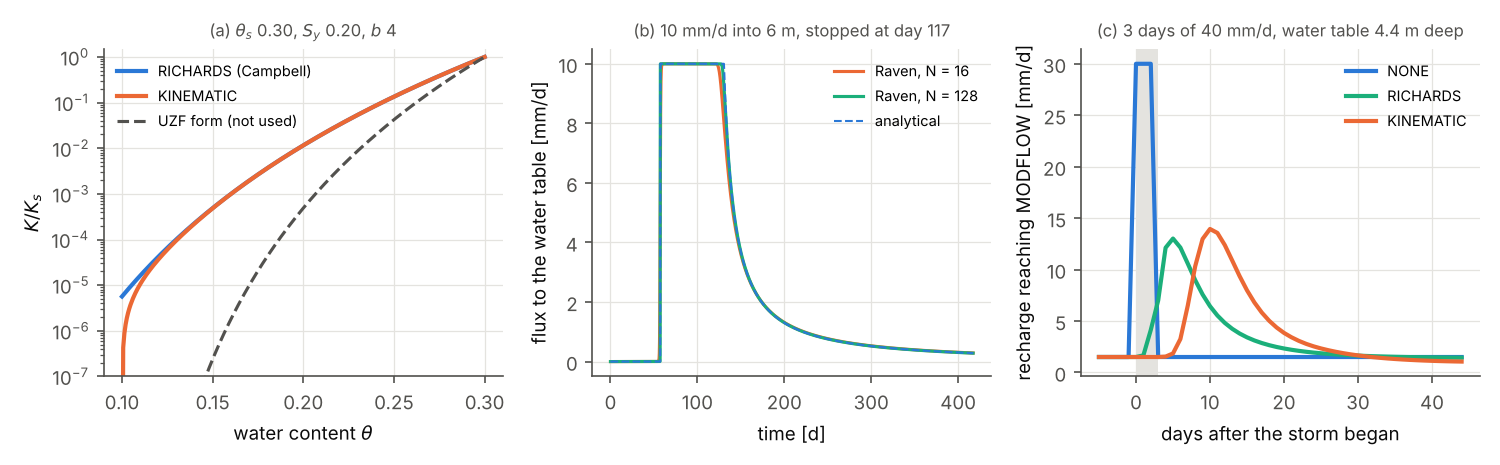
\includegraphics[width=\textwidth]{figures/fig_vz_kinematic.png}
\caption{\cmd{:SoilZoneVadose KINEMATIC}. (a) Conductivity (\ref{eq:kwK}) against Campbell's curve of \cmd{RICHARDS}
and the UZF form. (b) Test K1: flux into the water table of a 6~m column (sand, $K_s$ 0.5~m/d) under 10~mm/d from day 0
to 117, against the analytical kinematic wave (shock, then rarefaction). (c) Test K2: a 3-day storm of 40~mm/d after 400
days of 2~mm/d over a water table 4.4~m below the soil-zone base.}\label{fig:vzkinematic}
\end{figure}

\paragraph{Verification} (\cmd{test\_vz\_kinematic.py}, Section~\ref{ch:verification}).
K1, unit tests (167 checks): over 16\,000 random steps (materials, layers, fluxes, step lengths, \cmd{SPEC\_YIELD} 0) the
balance closes to $10^{-12}$ relative and every content stays within $[\theta_r,\theta_s]$. Against the analytical wave of
Figure~\ref{fig:vzkinematic}b (arrival on day 57.21) the flux reaches half its value on day 57.23 with 16 nodes and 57.21 with
128; the largest error of the drainage tail falls from 5.2\% of $q$ (16 nodes) through 2.7, 1.3 to 0.7\% (128 nodes); with
the default grid, accuracy and daily steps the arrival is 0.5\% late.
K2, the P1 storm: with the columns wetted by 400 days of 2~mm/d, the centroid of the storm's recharge reaches MODFLOW
7.6~days later with \cmd{RICHARDS} and 11.9~days later with \cmd{KINEMATIC}, at a similar peak (921 and 995~m$^3$/d
against 2\,280 without a column; Figure~\ref{fig:vzkinematic}c): without capillarity the front stays sharp and the
mobile water starts lower. Started at rest, as in test P1, the kinematic columns start at $\theta_r$ and soak up the
storm (centroid 72 days later, 15\% of it delivered in 90 days), whereas the Richards columns start at the wetter
hydrostatic profile (9.6 days).
K3 to K6: a water table rising through the column into the soil zone and falling again (the column goes and re-forms),
sand over clay with the water table rising through both, a hotstart continuity check and an existing-model round trip
(flows within $3\times10^{-5}$ of the generated model's); every balance at the standard limits, the column identity of
\cmd{sz\_check} from the first step. K9: the same outputs with a column leak of $10^{-5}$ or $10^{-4}$~m$^3$ per step
written into \cmd{GWBudget.csv} fail these checks.

\paragraph{Cost.} About 3 Newton iterations per node and substep; one 16-node column step costs 7 to 12~$\mu$s against
25 to 30~$\mu$s for \cmd{RICHARDS} on the same machine (unit test K1, timings machine-dependent).

\paragraph{Limits.} No capillarity: no upward redistribution inside the column, no capillary fringe above the water
table, and a sharp wetting front (the real one is smoother). The drained start $\theta_r$ is drier than a real
unsaturated zone: without \cmd{:SoilZoneVadoseInitialFlux} the first recharge of a run wets the columns before any of it
arrives (a few hundred days of 2~mm/d over a few metres). The reference makes the column consistent with MODFLOW's
$S_y$ by construction; a perched water table above a slow layer appears as saturated nodes that back up, not as a
pressure head.

\begin{refcard}{\cmd{:SoilZoneVadose KINEMATIC}}
\cmd{:SoilZoneVadose KINEMATIC} [$\epsilon$ [$N$]] in the \cmd{.rvg} file, with \cmd{:SoilZone PHYSICAL}.
$\epsilon$: largest content change in a substep, (0, 0.2], default 0.02; $N$: nodes per column at most, 3 to 200,
default 16. Materials per MODFLOW layer: \cmd{K\_VERT}, \cmd{POROSITY} ($\theta_s>0$, $\ge$ \cmd{SPEC\_YIELD}),
\cmd{SPEC\_YIELD}, \cmd{CLAPP\_B} (existing models: the model's K33/K and SY, retention of
\cmd{:SoilZoneAquiferClass}). Reference $\theta_s-S_y$; capillary rise from the water table (on by default,
\cmd{:SoilZoneCapillaryRise}); hotstart \cmd{:GWVadoseColumns}.
\end{refcard}
